\begin{figure}[H]
\begin{center}
\begin{adjustbox}{width=\columnwidth}
  
    \tikzset{every picture/.style={line width=0.75pt}}     
    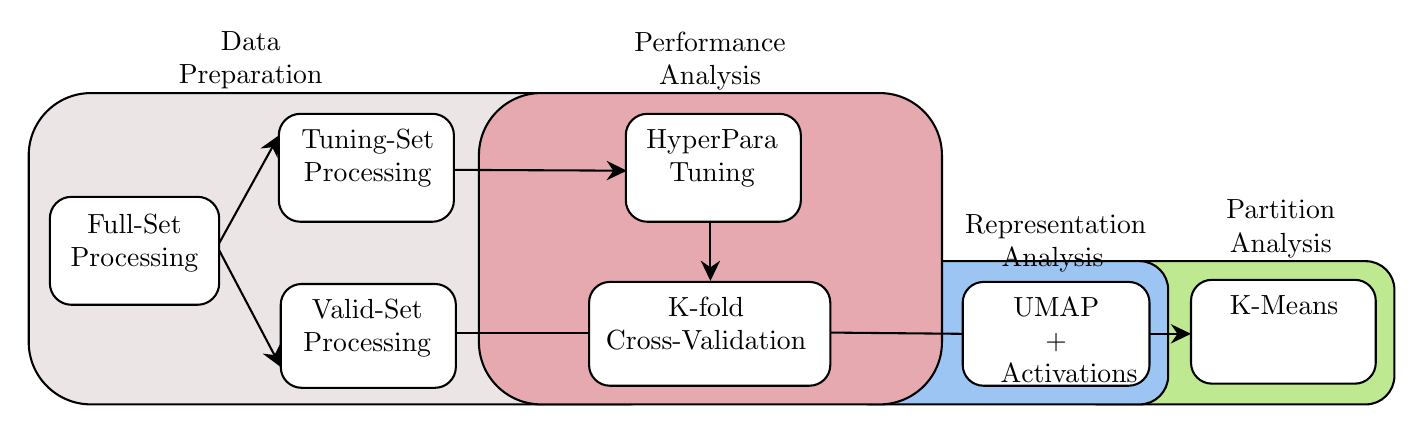
\begin{tikzpicture}[x=0.75pt,y=0.75pt,yscale=-1,xscale=1]
    %Rounded Rect [id:dp8958349243904878] 
    \draw  [fill={rgb, 255:red, 191; green, 233; blue, 145 }  ,fill opacity=1 ] (502.67,204.13) .. controls (502.67,196.51) and (508.85,190.33) .. (516.47,190.33) -- (644.87,190.33) .. controls (652.49,190.33) and (658.67,196.51) .. (658.67,204.13) -- (658.67,245.53) .. controls (658.67,253.15) and (652.49,259.33) .. (644.87,259.33) -- (516.47,259.33) .. controls (508.85,259.33) and (502.67,253.15) .. (502.67,245.53) -- cycle ;
    %Rounded Rect [id:dp32087219490227115] 
    \draw  [fill={rgb, 255:red, 235; green, 229; blue, 229 }  ,fill opacity=1 ] (0.67,139.33) .. controls (0.67,122.76) and (14.1,109.33) .. (30.67,109.33) -- (288.67,109.33) .. controls (305.24,109.33) and (318.67,122.76) .. (318.67,139.33) -- (318.67,229.33) .. controls (318.67,245.9) and (305.24,259.33) .. (288.67,259.33) -- (30.67,259.33) .. controls (14.1,259.33) and (0.67,245.9) .. (0.67,229.33) -- cycle ;
    %Rounded Rect [id:dp40803935509330935] 
    \draw  [fill={rgb, 255:red, 157; green, 197; blue, 244 }  ,fill opacity=1 ] (392.67,204.13) .. controls (392.67,196.51) and (398.85,190.33) .. (406.47,190.33) -- (535.87,190.33) .. controls (543.49,190.33) and (549.67,196.51) .. (549.67,204.13) -- (549.67,245.53) .. controls (549.67,253.15) and (543.49,259.33) .. (535.87,259.33) -- (406.47,259.33) .. controls (398.85,259.33) and (392.67,253.15) .. (392.67,245.53) -- cycle ;
    %Rounded Rect [id:dp9853366838815166] 
    \draw  [fill={rgb, 255:red, 230; green, 169; blue, 176 }  ,fill opacity=1 ] (217.58,139.33) .. controls (217.58,122.76) and (231.01,109.33) .. (247.58,109.33) -- (410.67,109.33) .. controls (427.24,109.33) and (440.67,122.76) .. (440.67,139.33) -- (440.67,229.33) .. controls (440.67,245.9) and (427.24,259.33) .. (410.67,259.33) -- (247.58,259.33) .. controls (231.01,259.33) and (217.58,245.9) .. (217.58,229.33) -- cycle ;
    %Straight Lines [id:da5215405961312622] 
    \draw    (91.51,183.33) -- (119.72,132.36) ;
    \draw [shift={(121.17,129.73)}, rotate = 478.96] [fill={rgb, 255:red, 0; green, 0; blue, 0 }  ][line width=0.08]  [draw opacity=0] (9.82,-4.72) -- (0,0) -- (9.82,4.72) -- (6.52,0) -- cycle    ;
    %Rounded Rect [id:dp7107992034558334] 
    \draw  [fill={rgb, 255:red, 255; green, 255; blue, 255 }  ,fill opacity=1 ] (121.17,129.73) .. controls (121.17,123.99) and (125.83,119.33) .. (131.57,119.33) -- (195.13,119.33) .. controls (200.87,119.33) and (205.53,123.99) .. (205.53,129.73) -- (205.53,160.93) .. controls (205.53,166.68) and (200.87,171.33) .. (195.13,171.33) -- (131.57,171.33) .. controls (125.83,171.33) and (121.17,166.68) .. (121.17,160.93) -- cycle ;
    %Rounded Rect [id:dp07619982590243402] 
    \draw  [fill={rgb, 255:red, 255; green, 255; blue, 255 }  ,fill opacity=1 ] (122.1,211.33) .. controls (122.1,205.81) and (126.58,201.33) .. (132.1,201.33) -- (196.46,201.33) .. controls (201.98,201.33) and (206.46,205.81) .. (206.46,211.33) -- (206.46,241.33) .. controls (206.46,246.86) and (201.98,251.33) .. (196.46,251.33) -- (132.1,251.33) .. controls (126.58,251.33) and (122.1,246.86) .. (122.1,241.33) -- cycle ;
    %Straight Lines [id:da2060512790122222] 
    \draw    (91.51,183.33) -- (120.7,238.68) ;
    \draw [shift={(122.1,241.33)}, rotate = 242.19] [fill={rgb, 255:red, 0; green, 0; blue, 0 }  ][line width=0.08]  [draw opacity=0] (9.82,-4.72) -- (0,0) -- (9.82,4.72) -- (6.52,0) -- cycle    ;
    %Rounded Rect [id:dp8467763959325827] 
    \draw  [fill={rgb, 255:red, 255; green, 255; blue, 255 }  ,fill opacity=1 ] (288.34,129.73) .. controls (288.34,123.99) and (293,119.33) .. (298.74,119.33) -- (362.29,119.33) .. controls (368.04,119.33) and (372.69,123.99) .. (372.69,129.73) -- (372.69,160.93) .. controls (372.69,166.68) and (368.04,171.33) .. (362.29,171.33) -- (298.74,171.33) .. controls (293,171.33) and (288.34,166.68) .. (288.34,160.93) -- cycle ;
    %Straight Lines [id:da6087855044000836] 
    \draw    (205.53,146.33) -- (285.87,146.72) ;
    \draw [shift={(288.87,146.73)}, rotate = 180.28] [fill={rgb, 255:red, 0; green, 0; blue, 0 }  ][line width=0.08]  [draw opacity=0] (9.82,-4.72) -- (0,0) -- (9.82,4.72) -- (6.52,0) -- cycle    ;
    %Rounded Rect [id:dp36167370728246717] 
    \draw  [fill={rgb, 255:red, 255; green, 255; blue, 255 }  ,fill opacity=1 ] (270.65,210.33) .. controls (270.65,204.81) and (275.13,200.33) .. (280.65,200.33) -- (376.87,200.33) .. controls (382.39,200.33) and (386.87,204.81) .. (386.87,210.33) -- (386.87,240.33) .. controls (386.87,245.86) and (382.39,250.33) .. (376.87,250.33) -- (280.65,250.33) .. controls (275.13,250.33) and (270.65,245.86) .. (270.65,240.33) -- cycle ;
    %Straight Lines [id:da44361816804799015] 
    \draw    (205.87,224.73) -- (270.87,224.73) ;
    %Rounded Rect [id:dp4735015562322822] 
    \draw  [fill={rgb, 255:red, 255; green, 255; blue, 255 }  ,fill opacity=1 ] (10.86,169.73) .. controls (10.86,163.99) and (15.52,159.33) .. (21.26,159.33) -- (82.04,159.33) .. controls (87.78,159.33) and (92.44,163.99) .. (92.44,169.73) -- (92.44,200.93) .. controls (92.44,206.68) and (87.78,211.33) .. (82.04,211.33) -- (21.26,211.33) .. controls (15.52,211.33) and (10.86,206.68) .. (10.86,200.93) -- cycle ;
    %Straight Lines [id:da8145463847735959] 
    \draw    (329.12,170.83) -- (329.12,196.83) ;
    \draw [shift={(329.12,199.83)}, rotate = 270] [fill={rgb, 255:red, 0; green, 0; blue, 0 }  ][line width=0.08]  [draw opacity=0] (9.82,-4.72) -- (0,0) -- (9.82,4.72) -- (6.52,0) -- cycle    ;
    %Rounded Rect [id:dp6977268643716749] 
    \draw  [fill={rgb, 255:red, 255; green, 255; blue, 255 }  ,fill opacity=1 ] (450.67,210.33) .. controls (450.67,204.81) and (455.14,200.33) .. (460.67,200.33) -- (530.67,200.33) .. controls (536.19,200.33) and (540.67,204.81) .. (540.67,210.33) -- (540.67,240.33) .. controls (540.67,245.86) and (536.19,250.33) .. (530.67,250.33) -- (460.67,250.33) .. controls (455.14,250.33) and (450.67,245.86) .. (450.67,240.33) -- cycle ;
    %Rounded Rect [id:dp7890525886281983] 
    \draw  [fill={rgb, 255:red, 255; green, 255; blue, 255 }  ,fill opacity=1 ] (560.67,209.33) .. controls (560.67,203.81) and (565.14,199.33) .. (570.67,199.33) -- (639.67,199.33) .. controls (645.19,199.33) and (649.67,203.81) .. (649.67,209.33) -- (649.67,239.33) .. controls (649.67,244.86) and (645.19,249.33) .. (639.67,249.33) -- (570.67,249.33) .. controls (565.14,249.33) and (560.67,244.86) .. (560.67,239.33) -- cycle ;
    %Straight Lines [id:da5635979583415296] 
    \draw    (386.87,224.73) -- (450.67,225.33) ;
    %Straight Lines [id:da6185748663159079] 
    \draw    (540.67,225.33) -- (557.67,225.33) ;
    \draw [shift={(560.67,225.33)}, rotate = 180] [fill={rgb, 255:red, 0; green, 0; blue, 0 }  ][line width=0.08]  [draw opacity=0] (9.82,-4.72) -- (0,0) -- (9.82,4.72) -- (6.52,0) -- cycle    ;
    
    % Text Node
    \draw (16.96,166) node [anchor=north west][inner sep=0.75pt]   [align=left] {\begin{minipage}[lt]{49.730644000000005pt}\setlength\topsep{0pt}
    \begin{center}
    {\fontfamily{lms}\selectfont Full-Set}\\

    {\fontfamily{lms}\selectfont Processing}
    \end{center}
    
    \end{minipage}};
    % Text Node
    \draw (128.04,125.33) node [anchor=north west][inner sep=0.75pt]   [align=left] {\begin{minipage}[lt]{51.714pt}\setlength\topsep{0pt}
    \begin{center}
    {\fontfamily{lms}\selectfont Tuning-Set}\\

    {\fontfamily{lms}\selectfont Processing}
    \end{center}
    
    \end{minipage}};
    % Text Node
    \draw (274.53,206) node [anchor=north west][inner sep=0.75pt]   [align=left] {\begin{minipage}[lt]{76.47756000000001pt}\setlength\topsep{0pt}
    \begin{center}
    {\fontfamily{lms}\selectfont K-fold}\\
    
    {\fontfamily{lms}\selectfont Cross-Validation}
    \end{center}
    
    \end{minipage}};
    % Text Node
    \draw (129.11,207.33) node [anchor=north west][inner sep=0.75pt]   [align=left] {\begin{minipage}[lt]{49.730644000000005pt}\setlength\topsep{0pt}
    \begin{center}
    {\fontfamily{lms}\selectfont Valid-Set}\\

    {\fontfamily{lms}\selectfont Processing}
    \end{center}
    
    \end{minipage}};
    % Text Node
    \draw (294.35,125.33) node [anchor=north west][inner sep=0.75pt]   [align=left] {\begin{minipage}[lt]{51.056644pt}\setlength\topsep{0pt}
    \begin{center}
    {\fontfamily{lms}\selectfont HyperPara}\\

    {\fontfamily{lms}\selectfont Tuning}
    \end{center}
    
    \end{minipage}};
    % Text Node
    \draw (467.43,206.33) node [anchor=north west][inner sep=0.75pt]   [align=left] {\begin{minipage}[lt]{40.199356pt}\setlength\topsep{0pt}
    \begin{center}
    {\fontfamily{lms}\selectfont UMAP}\\
    {\fontfamily{lms}\selectfont + }\\
    {\fontfamily{lms}\selectfont Activations}
    \end{center}
    
    \end{minipage}};
    % Text Node
    \draw (285.33,78.33) node [anchor=north west][inner sep=0.75pt]   [align=left] {\begin{minipage}[lt]{63.18335600000001pt}\setlength\topsep{0pt}
    \begin{center}
    {\fontfamily{lms}\selectfont Performance}\\
    {\fontfamily{lms}\selectfont Analysis}
    \end{center}
    
    \end{minipage}};
    % Text Node
    \draw (52.16,78.33) node [anchor=north west][inner sep=0.75pt]   [align=left] {\begin{minipage}[lt]{80.92pt}\setlength\topsep{0pt}
    \begin{center}
    {\fontfamily{lms}\selectfont Data}\\
    {\fontfamily{lms}\selectfont Preparation}
    \end{center}
    
    \end{minipage}};
    % Text Node
    \draw (575.5,205.33) node [anchor=north west][inner sep=0.75pt]   [align=left] {\begin{minipage}[lt]{42.783356000000005pt}\setlength\topsep{0pt}
    \begin{center}
    {\fontfamily{lms}\selectfont K-Means}
    \end{center}
    
    \end{minipage}};
    % Text Node
    \draw (450.33,159.33) node [anchor=north west][inner sep=0.75pt]   [align=left] {\begin{minipage}[lt]{63.18335600000001pt}\setlength\topsep{0pt}
    \begin{center}
    {\fontfamily{lms}\selectfont Representation}\\
    {\fontfamily{lms}\selectfont Analysis}
    \end{center}
    
    \end{minipage}};
    % Text Node
    \draw (560.33,159.33) node [anchor=north west][inner sep=0.75pt]   [align=left] {\begin{minipage}[lt]{63.18335600000001pt}\setlength\topsep{0pt}
    \begin{center}
    {\fontfamily{lms}\selectfont Partition}\\
    {\fontfamily{lms}\selectfont Analysis}
    \end{center}
    
    \end{minipage}};
    \end{tikzpicture}
\end{adjustbox}
\end{center}
\caption[\textbf{Experimental Pipeline}]{Arrows indicate the flow of the pipeline. Big coloured blocks are major pipeline steps, white rectangles indicate sub-tasks within each step.}
\label{fig: pipeline}
\end{figure}